%----------------------------------------------------------------------------
\chapter{Megoldók ismertetése és összehasonlítása}
%----------------------------------------------------------------------------

\section{Megoldó MATLAB környezetben}
Mint minden fizikai modellnek, ennek is verifikálhatónak kell lennie, mivel csak
így lehet megbízni benne.
A  verifikálásra egy 1D-s problémát állítottam össze.
A "rúd" két végén hasonlóan $\varphi_0=0$ és $\varphi_0=1$ Dirichlet feltételt írtam elő.
Ennek a problémának létezik analitikus megoldása, amihez a szimulátor eredménye megfelelő pontossággal konvergál.
A következő ábrán látható a megoldás eredménye: az villamos potenciál eloszlása és az 
elektromos tér nagysága
\begin{figure}[H]
\centering
%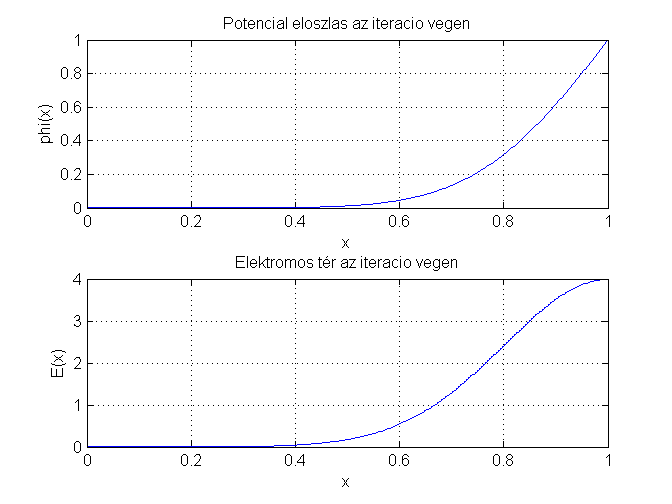
\includegraphics[width=100mm, keepaspectratio]{figures/feszko1.png}
\caption{1D-s probléma megoldása} 
%\label{fig:equivTV}
\end{figure}
\newpage

\noindent Az iteráció során a megoldás konvergálását a következő ábrán láthatjuk:
\begin{figure}[H]
\centering
%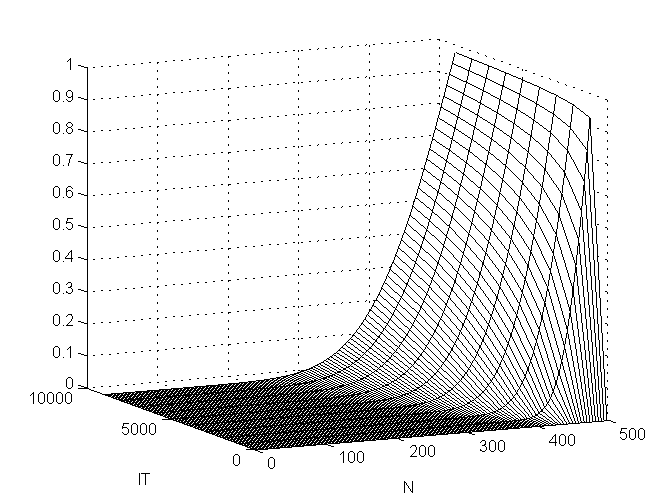
\includegraphics[width=100mm, keepaspectratio]{figures/feszko2.png}
\caption{1D-s probléma ereményének iteráció soráni változása} 
%\label{fig:equivTV}
\end{figure}
Megfigyelhető, hogy egy adott iteráció szám után lényegesen nem változik a megoldás, amikor is
a szimulációt leállíthattuk volna.\\


\noindent A korábbiakban ismertetett 2D-s problémára analóg módon kiterjesztettem a szimulátort,
aminek lefuttatása után a következő potenciáleloszlást kaptam:
\begin{figure}[H]
\centering
%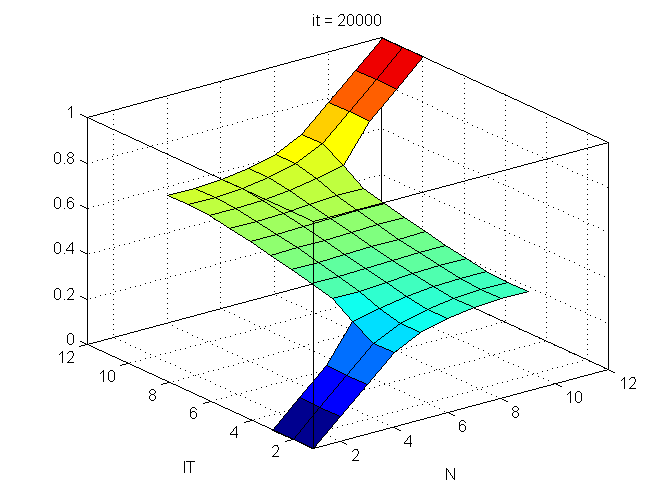
\includegraphics[width=100mm, keepaspectratio]{figures/2dfeszko2.png}
\caption{2D-s probléma eredménye} 
%\label{fig:equivTV}
\end{figure}
\newpage

\noindent A MATLAB környezetbeli szimulátorok felépítése során törekedtem arra,
hogy a CUDA platformra történő portolási folyamat könnyen kivitelezhető legyen.
Nem használtam különleges MATLAB függvényeket, se Toolboxok függvényeit.

\section{Megoldó CUDA-C nyelven}
A vizsgált tartomány pontjait blokkokba kell rendezni a korábbiaknak megfelelően.
Az egyszerűség kedvéért a tartományt a futtatható szálak egész számú többszöröse
mínusz 2 pontra bontom fel.
\begin{figure}[H]
\centering
%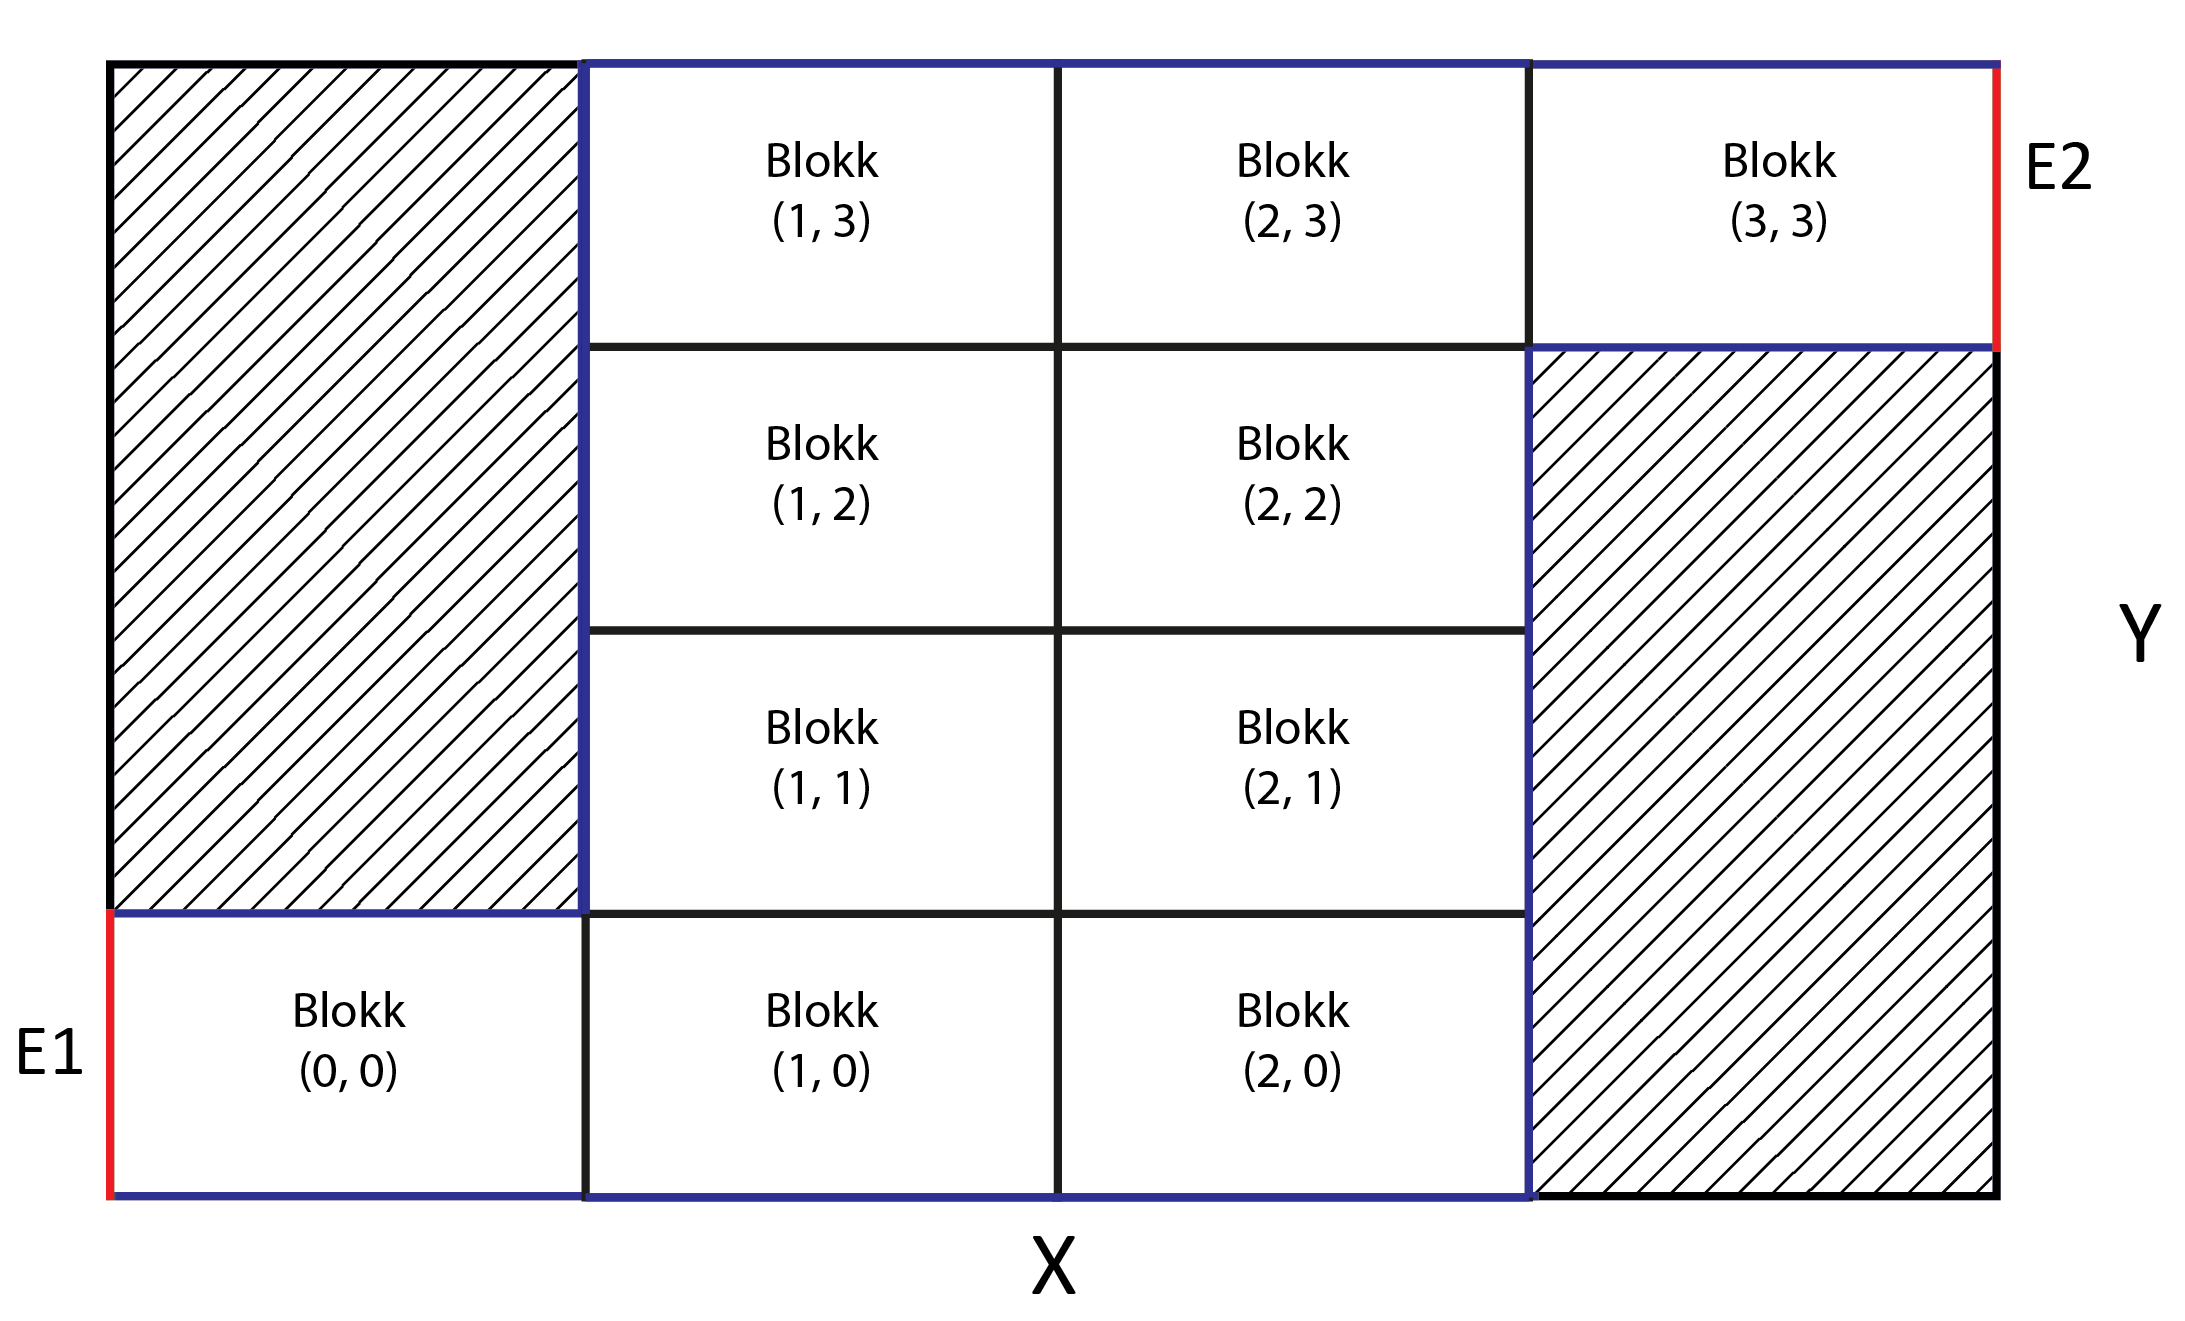
\includegraphics[width=100mm, keepaspectratio]{figures/domCUDA.png}
\caption{A tartomány felosztása párhuzamosításra} 
%\label{fig:equivTV}
\end{figure}
A szimuláció során egy pont értéke a szomszédos pontok korábbi értékeitől is függenek.
Ennek megfelelően szükséges ez a plussz két sor és oszlop.
A párhuzamos szimuláció során a egy iteráció után szinkronizálni kell a szálakat és "kicserélni"
a blokkok szélén lévő pontok értékeit.
Ez egy természetes dolog, ha nagyobb és speciálisabb szimulációt végzünk.

\section{Összehasonlítás}
A két megoldó számértékeileg azonos értékre jut. Ezt vártuk az azonos IEEE 754-es szabvány
megvalósítása végett. CPU-n $389.3 ms$-ig tartott a szimulátor magjának futása, míg a GPU-n 
$9.4 ms$-ig tartott. Ez $\sim 40 \times$ gyorsulást jelent.
